% ------------------------------------------------------------------------------
% TYPO3 v9 LTS - What's New (German Version)
%
% @license	Creative Commons BY-NC-SA 3.0
% @link		https://typo3.org/help/documentation/whats-new/
% @language	German
% ------------------------------------------------------------------------------

\section{Suchmaschinenoptimierung}
\begin{frame}[fragile]
	\frametitle{Suchmaschinenoptimierung}

	\begin{center}\huge{\color{typo3darkgrey}\textbf{Suchmaschinenoptimierung}}\end{center}
	\begin{center}\large{\textit{Now we can "SEO" you}}\end{center}

\end{frame}

% ------------------------------------------------------------------------------

\begin{frame}[fragile]
	\frametitle{Suchmaschinenoptimierung}
	\framesubtitle{Suchmaschinenoptimierung}

	Die Seiteneigenschaften verfügen über einen neuen Tab "SEO", mit dem BE-Benutzer
	SEO-bezogene Informationen, \href{http://ogp.me/}{Open Graph}-Daten und vieles mehr konfigurieren können.

	\begin{figure}
		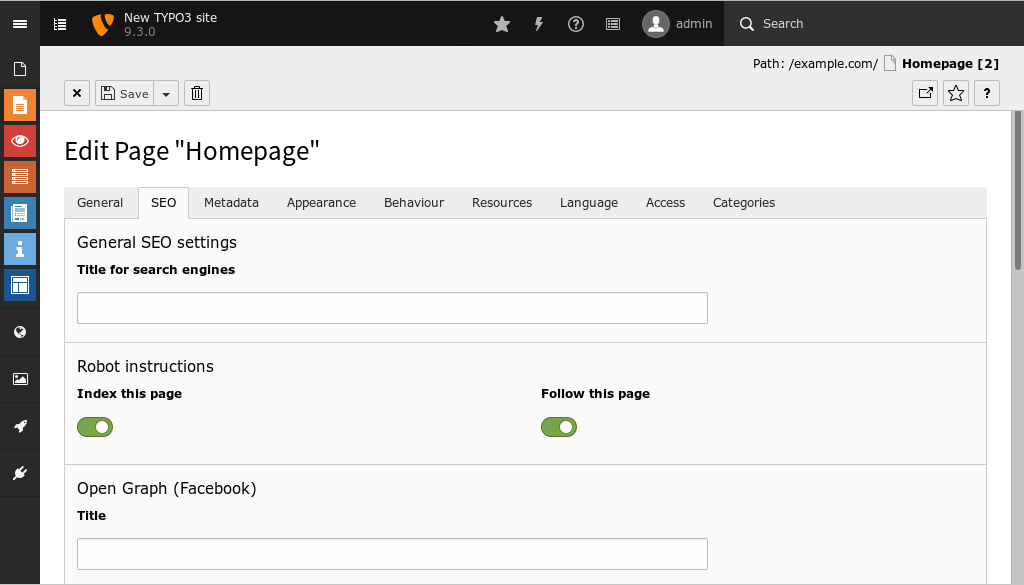
\includegraphics[width=0.70\linewidth]{SearchEngineOptimization/SearchEngineOptimizationPageProperties.png}
	\end{figure}

\end{frame}

% ------------------------------------------------------------------------------

\begin{frame}[fragile]
	\frametitle{Suchmaschinenoptimierung}
	\framesubtitle{Suchmaschinenoptimierung (SEO)}

	\begin{itemize}
		\item Die neue
			\href{https://docs.typo3.org/typo3cms/CoreApiReference/ApiOverview/PageTitleApi/Index.html}{Page Title API}
			ermöglicht Integratoren und Entwicklern zu beeinflussen, was genau als Seitentitel
			angezeigt wird
		\item TYPO3 kann nun
			\href{https://docs.typo3.org/typo3cms/CoreApiReference/ApiOverview/XmlSitemap/Index.html}{XML Sitemaps}
			generieren, mit der Möglichkeit verschiedene Sitemaps pro Website und pro Sprache
			wiederzugeben
		\item Kanonische Links werden zu den Seiten automatisch hinzugefügt, um 
			Ranking-Strafen aufgrund von doppeltem Inhalt zu vermeiden
		\item In mehrsprachigen TYPO3-Sites werden \texttt{hreflang}-Tags automatisch
			hinzugefügt
		\item SEO-bezogene Meta-Tags, die in den Seiteneigenschaften festgelegt sind, werden jetzt standardmäßig 
			im Frontend gerendert

	\end{itemize}

\end{frame}

% ------------------------------------------------------------------------------
% Meta Tag Manager (API)
% #81464 - Add API for meta tag management

\begin{frame}[fragile]
	\frametitle{Suchmaschinenoptimierung}
	\framesubtitle{Meta-Tag-Manager}

	% decrease font size for code listing
	\lstset{basicstyle=\tiny\ttfamily}

	\begin{itemize}
		\item Die neue
			\href{https://docs.typo3.org/typo3cms/CoreApiReference/ApiOverview/MetaTagApi/Index.html}{Meta-Tag API}
			wurde zum Verwalten und Rendern der Metatags auf flexible,
			geregelte Weise eingeführt
		\item TYPO3 Core liefert zum Beispiel einen \href{http://ogp.me/}{Open Graph}
			Meta Tag Manager:

\begin{lstlisting}
use \TYPO3\CMS\Core\MetaTag\MetaTagManagerRegistry;
$metaTagManager = MetaTagManagerRegistry::getInstance()->getManagerForProperty('og:title');
$metaTagManager->addProperty('og:title', 'This is the OG title from a controller');
\end{lstlisting}

		\item Weitere verfügbare Beispielsfunktionen:

			\begin{itemize}
				\smaller
					\item \texttt{\$metaTagManager->addProperty()}
					\item \texttt{\$metaTagManager->removeProperty()}
					\item \texttt{\$metaTagManager->removeAllProperties()}
			\end{itemize}

	\end{itemize}

\end{frame}

% ------------------------------------------------------------------------------
% Meta Tag Manager (API)
% #81464 - Add API for meta tag management

\begin{frame}[fragile]
	\frametitle{Suchmaschinenoptimierung}
	\framesubtitle{Meta-Tag-Manager}

	% decrease font size for code listing
	\lstset{basicstyle=\tiny\ttfamily}

	\begin{itemize}
		\item Entwickler können benutzerdefinierte \texttt{MetaTagManager} in der
			\texttt{MetaTagManagerRegistry} anlegen

\begin{lstlisting}
use \TYPO3\CMS\Core\MetaTag\MetaTagManagerRegistry;
$metaTagManagerRegistry = MetaTagManagerRegistry::getInstance();
$metaTagManagerRegistry->registerManager(
  'custom',
  \Some\CustomExtension\MetaTag\CustomMetaTagManager::class
);
\end{lstlisting}

		\item Meta-Tags können mit TypoScript und PHP gesetzt werden

\begin{lstlisting}
page.meta {
  og:site_name = TYPO3
  og:site_name.attribute = property
  og:site_name.replace = 1
}
\end{lstlisting}

			\smaller
				("\texttt{replace = 1}" ersetzt zuvor festgelegte Meta-Tags)
			\normalsize

	\end{itemize}

\end{frame}

% ------------------------------------------------------------------------------
